\begin{figure}
    \centering
    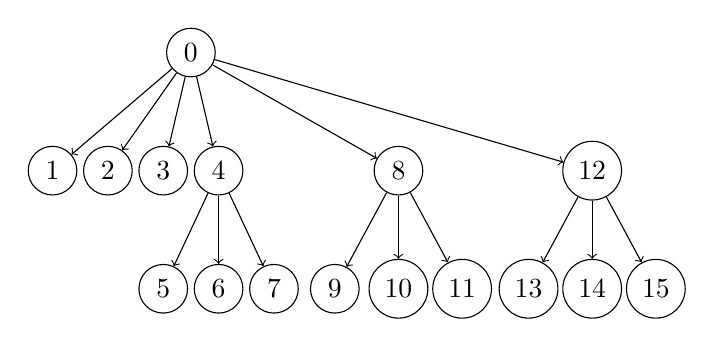
\begin{tikzpicture} [every node/.style = {shape=circle, draw, align=center}]
        % \tikzstyle{level 1}=[sibling distance=4em]
        % \tikzstyle{level 2}=[sibling distance=2em]
        \node {0}
        child [->, sibling distance=2em] { node {1}}
        child [->, sibling distance=2em] { node {2}}
        child [->, sibling distance=2em] { node {3}}
        child  [->, sibling distance=2em] { node {4}
            child [sibling distance=2em] {node {5}}
            child [sibling distance=2em] {node {6}}
            child [sibling distance=2em] {node {7}}
        }
        child [->, sibling distance=5em] { node {8}
            child [sibling distance=2.3em] {node {9}}
            child [sibling distance=2.3em] {node {10}}
            child [sibling distance=2.3em] {node {11}}
        }
        child [->, sibling distance=5.8em] { node {12}
            child [sibling distance=2.3em] {node {13}}
            child [sibling distance=2.3em] {node {14}}
            child [sibling distance=2.3em] {node {15}}
        };


    \end{tikzpicture}
    \caption{16 processes structured in a Knomial tree with radix four. Each message is the same size.}
    \label{fig:graph-knomial}
\end{figure}